\chapter{Continuous Models}
Many engineered systems consist of computers, communications networks, and other digital (i.e., discrete event) systems whose purpose is to monitor and control a physical (electrical, mechanical, thermodynamic, etc.) process. Models of these systems have parts modeled as discrete event systems, parts modeled with continuous (differential or differential-algebraic) equations, and the interaction of these parts is crucial to understanding the system's behavior. Where the continuous models interact with the discrete event models, these interactions are necessarily discrete. For example, a digital thermometer reports temperature in discrete increments, electrical switches are either open or closed, a threshold sensor is either tripped or it is not. Discrete interactions in a combined continuous-discrete event simulation are managed just as before; the models interact by producing output events and reacting to input events.

If, on the other hand, two systems interact continuously, then those interacting parts at least are modeled with continuous equations. In this case, accurate simulation is greatly facilitated by lumping the two systems into a single assembly; in \adevs\ this assembly is an \classname{Atomic} model that encapsulates the system's continuous dynamics. The essence of the approach to combined simulation in \adevs\ consists therefore of building atomic models that i) approximate the behavior of the continuous systems and ii) generates and consumes events at those instants when the continuous system interacts with a discrete event one.

There are three possibly outcomes of this lumping process. One possibility is that we end up with a single assembly; in this case our model is essentially continuous and we are probably better off using a simulation tool for continuous systems. At the other extreme, we find that the continuous parts of our model are very simple, yielding to analytical solutions that are easily transformed into discrete event models. Between these two extremes are models with continuous dynamics that are not simple but also do not dominate the modeling problem. The continuous system simulation part of \adevs\ is aimed at this type of model.

\section{Differential equation modeling with the \classname{ode\_system} class}
Models described by ordinary differential equations are implemented by sub-classing the \classname{ode\_system} class. This class has two sets of methods: the first is for the model's continuous dynamics and the second is for the model's discrete event dynamics. I'll illustrate both with the simple, if somewhat contrived, example of a cherry bomb\footnote{A cherry bomb is a small red firecracker. They are dangerous, and illegal in the United States. Nonetheless, every school seems to have at least one obnoxious kid who likes to put them into toilets.}. This bomb is dropped from a height of 1 meter and bounces until it either explodes or is doused with water. We'll assume that the cherry bomb only bounces up and down and is perfectly elastic. The cherry bomb explodes 2 seconds from the time it is lit and dropped unless doused first. Dousing the cherry bomb puts out the fuse\footnote{Cherry bomb fuses are frequently water proofed.}. Dousing is a discrete input event and the cherry bomb produces a discrete output event if it explodes. 

This model has two continuous state variables: the height and velocity of the cherry bomb. Between events, these variables are governed by the pair of differential equations
\begin{align}
&\dot{v} = -9.8 \label{eqn:v} \\
&\dot{h} = v \label{eqn:h}
\end{align}
where $9.8$ meters per second per second is acceleration due to gravity, $v$ is velocity, and $h$ is height. In this example, it is also useful to know the current time. We keep track of this by adding one more differential equation
\begin{equation}
\dot{t} = 1 \label{eqn:t}
\end{equation}
whose solution is $t_0 + t$ or just $t$ if we set $t_0 = 0$. The ball bounces when it hits the floor, and bouncing causes the ball's velocity to change sign; specifically
\begin{equation}
h = 0 \ \& \ v < 0 \implies v \leftarrow -v \label{eqn:state_event}
\end{equation}
where $\implies$ is logical implication and $\leftarrow$ indicates an assignment. 

Equations \ref{eqn:v}, \ref{eqn:h}, and \ref{eqn:t} are the state variable derivatives, and these equations are implemented in the \methodname{der\_func} method of the \classname{ode\_system} class. The signature for this method is
\begin{verbatim}
void der_func(const double* q, double* dq)
\end{verbatim}
The q pointer is the array of state variable values; in this case $h$, $v$, and $t$. The dq pointer is the array of state variable derivatives; in this case $\dot{h}$, $\dot{v}$, and $\dot{t}$. When the simulator calls the der\_func method, it supplies q. In response, the method computes the values of $\dot{h}$, $\dot{q}$, and $\dot{t}$ and stores them in the dq array.

Equation \ref{eqn:state_event} is a state event condition and it is implemented in two parts. The \methodname{state\_event\_func} method implements the `if' part (left hand side) of the condition. The signature of this method is
\begin{verbatim}
void state_event_func(const double *q, double *z)
\end{verbatim}
Again, the supplied q array contains the current state variable values. These are used to evaluate the state event condition and store the result in the z array. The simulator detects state events by looking for changes in the sign of the z array entries. Note that the event condition should be continuous in the state variables on which it depends. In the case of the cherry bomb this is simple to do: we simply use $z=h$ if $v < 0$ and $z=1$ if $v >= 0$.  

The `then' part (right hand side) is implemented with the \methodname{internal\_event} method, which the simulator invokes when the state event condition is true. The signature of this method is
\begin{verbatim}
void internal_event(double *q, const bool *state_event)
\end{verbatim}
where, again, $q$ is the value of the state variables at the event. The entries of the array state\_event are true for each z in the state event condition array that evaluates to zero. This array therefore has one entry for each state event condition, and it has one additional entry to indicate time events, which are described below.

The cherry bomb has one discrete state variable with three possible values: the fuse is lit, the fuse is not lit, and the bomb is exploded. This variable changes in response to two events. The first event is when the bomb explodes; this is a time event that we know will occur 2 seconds from the time that the fuse it lit. The \methodname{time\_event\_func} method is used to schedule the explosion by returning the time remaining until the fuse burns out. The signature of the of this method is
\begin{verbatim}
double time_event_func(const double* q)
\end{verbatim}
As before, q is the current value of the state variables. The \methodname{time\_event\_func} is similar to the familiar \methodname{ta} method; it is used to schedule autonomous events based on the current value of the model's state variables. When this time expires, the simulator calls the \methodname{internal\_event} method with the last flag in the state event array set to true.

The second event that can change the state of the fuse is dousing with water. This an external event. External events, of course, are not scheduled by the model itself; they occur when and if the input event arrives. The \methodname{external\_event} method implements the response of the cherry bomb to dousing with water. Its signature is
\begin{verbatim}
void external_event(double *q, double e, const Bag<X> &xb)
\end{verbatim}
The array q contains the values of the continuous state variables, e is the time since the last discrete event, and xb is the bag of input. The douse event is an input and it appears in the input bag xb if the event occurs. 

As before, it is possible for an external and internal event to coincide. When this happens, the simulator calls the method \methodname{confluent\_event}. Its signature is
\begin{verbatim}
void confluent_event (double *q, const bool *state_event, const Bag<X> &xb)
\end{verbatim}
and its arguments are as described for the internal and external methods.

The cherry bomb model produces an output event when it explodes, and the \methodname{output\_func} method is use for this purpose. Its signature is
\begin{verbatim}
void output_func(const double *q, const bool *state_event, Bag<X> &yb)
\end{verbatim}
Its q and state\_event arguments are as described for the internal\_event method, and the bag yb is to be filled with the model's output. As with an \classname{Atomic} model, the output\_func is always invoked immediately prior to the internal\_event and confluent\_event methods.

All that remains in the implementation is to supply a \methodname{gc\_output} for collecting garbage, a constructor, and a method for initializing the continuous state variables. The gc\_output method works identically to that of the \classname{Atomic} class and so needs no more discussion here. The constructor for the cherry bomb must call the constructor of its \classname{ode\_system} base class. The signature of this method is
\begin{verbatim}
ode_system (int N_vars, int M_event_funcs)
\end{verbatim}
where N\_vars is the number of entries in the q and dq arrays (i.e., the number of continuous state variables) and M\_event\_funcs is the number of entries in the z and state\_event arrays (plus one for the time event). For the cherry bomb, N\_vars is three and M\_event\_funcs is one.

The constructor does not initialize the continuous state variables. Instead, the simulator calls the init method whose signature is
\begin{verbatim}
void init(double* q)
\end{verbatim}
and where q is an array that should be filled with the initial values for, in the case of the cherry bomb, $h$, $v$, and $t$. The complete implementation of the \classname{CherryBomb} is listed below.
\begin{verbatim}
#include "adevs.h"
#include <iostream>
using namespace std;
using namespace adevs;

// Array indices for the CherryBomb state variables
#define H 0
#define V 1
#define T 2
// Discrete variable enumeration for the CherryBomb
typedef enum { FUSE_LIT, DOUSE, EXPLODE } Phase;

class CherryBomb: public ode_system<string> {
   public:
      CherryBomb():ode_system<string>(
            3, // three state variables including time
            1 // 1 state event condition
            ) {
         phase = FUSE_LIT; // Light the fuse!
      }
      void init(double *q) {
         q[H] = 1.0; // Initial height
         q[V] = 0.0; // Initial velocity
         q[T] = 0.0; // Start time at zero
      }
      void der_func(const double* q, double* dq) {
         dq[V] = -9.8; 
         dq[H] = q[V]; 
         dq[T] = 1.0; 
      }
      void state_event_func(const double* q, double *z) {
         // Test for hitting the ground. 
         if (q[V] < 0.0) z[0] = q[H];
         else z[0] = 1.0;
      }
      double time_event_func(const double* q) {
         if (q[T] < 2.0) return 2.0 - q[T]; // Explode at time 2
         else return DBL_MAX; // Don't do anything after that
      }
      void external_event(double* q, double e, const Bag<string>& xb) {
         phase = DOUSE; // Any input is a douse event
      }
      void internal_event(double* q, const bool* state_event) {
         if (state_event[0]) q[V] = -q[V]; // Bounce!
         if (state_event[1]) phase = EXPLODE;
      }
      void confluent_event(double* q, const bool* state_event,
         const Bag<string>& xb) {
         internal_event(q,state_event);
         external_event(q,0.0,xb);
      }
      void output_func(const double *q, const bool* state_event,
            Bag<string>& yb) {
         if (state_event[1] && phase == FUSE_LIT)
            yb.insert("BOOM!"); // Explode!
      }
      void postStep(const double* q) {
         // Write the current state to std out
         cout << q[T] << " " << q[H] << " " << q[V] << " " << phase << endl;
      }
      // No garbage collection is needed
      void gc_output(Bag<string>&){}
      // Get the current value of the discrete variable
      Phase getPhase() { return phase; } 
   private:
      Phase phase;
};
\end{verbatim}

The \classname{CherryBomb} itself is not derived from \classname{Atomic} and so cannot be simulated directly. Rather, it is given to a \classname{Hybrid} object, which is a kind of \classname{Atomic}, that generators the trajectories for the model. This \classname{Hybrid} object is used just like any other \classname{Atomic} model. Input to this \classname{Hybrid} object triggers an input event for the \classname{ode\_system} that is contains. Likewise, output from the \classname{ode\_system} becomes output from the \classname{Hybrid} object. Most importantly, the hybrid model can be part of any network of discrete event models.

A \classname{Hybrid} object is provided with three things when it is constructed. First is the \classname{ode\_system} itself. Second is an \classname{ode\_solver} that produces the model's continuous trajectories. \adevs\ has two types of \classname{ode\_solvers}: a \classname{corrected\_euler} solver that uses the corrected Euler method and a \classname{rk\_45} solver that uses a fourth order Runge-Kutta method. Third is an \classname{event\_locator} that finds the location of state events as the simulation progresses. \adevs\ has only one of these: the \classname{linear\_event\_locator}. The code below shows how these are used to create and simulate a \classname{Hybrid} object.
\begin{verbatim}
int main() {
   // Create the model
   CherryBomb* bomb = new CherryBomb();
   // Create the ODE solver for this model. Maximum error
   // tolerance at each step is 1E-4 and the maximum
   // size of an integration step is 0.01.
   ode_solver<string>* ode_solve =
      new corrected_euler<string>(bomb,1E-4,0.01);
   // Create the event locator for this model. Maximum
   // error tolerance for the location of an event in
   // the state space is 1E-8.
   event_locator<string>* event_find =
      new linear_event_locator<string>(bomb,1E-8);
   // Create an atomic model that puts all of these
   // together to simulate the continuous system.
   Hybrid<string>* model =
      new Hybrid<string>(bomb,ode_solve,event_find);
   // Create and run a simulator for this model
   Simulator<string>* sim = new Simulator<string>(model);
   while (bomb->getPhase() == FUSE_LIT)
      sim->execNextEvent();
   delete sim; delete bomb;
   return 0;
}

\end{verbatim}

Figure \ref{fig:cherry_bomb_trajectory} shows the cherry bomb's trajectory from $t=0$ to its explosion at $t=2$. This plot was produced using the simulation program listed above. There is nothing particular surprising about it, but you can observe the discrete changes in the cherry bomb's trajectory. There are two bounce events at $t \approx 0.45$ and $t \approx 1.4$. The cherry bomb explodes abruptly at the start of its third descent.
\begin{figure}[ht]
\centering
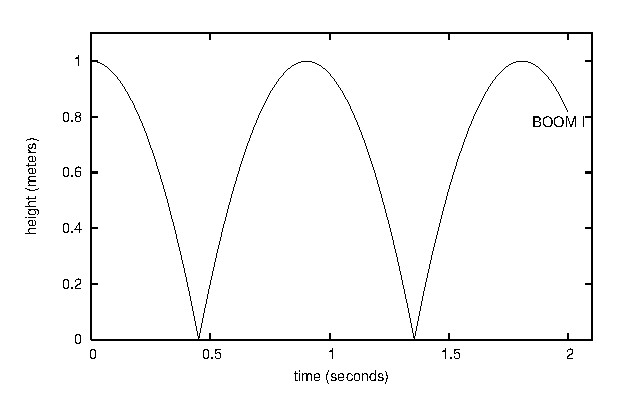
\epsfig{file=cont_models_figs/ball_height.eps}
\caption{A simulation of the cherry bomb model that terminates when the cherry bomb explodes.}
\label{fig:cherry_bomb_trajectory}
\end{figure}

\section{Modeling hybrid systems with adevs and OpenModelica}
It is possible to generate models in the form described above automatically from the Modelica programming language. This has several advantages, among them are:
\begin{enumerate}
\item You may be able to reuse large numbers of model components from the Modelica standard library.
\item Very complicated models, including differential-algebraic systems and models that difficult to initialize, may have code for the simulation automatically generated.
\item Modification of the continuous model will be much simpler in the future because the model description is separated from the problems of its simulation (these being handled automatically by the OpenModelica compiler and runtime system).
\end{enumerate}

To take advantage of the Modelica language, you will need to get and install from source the OpenModelica compiler, which is hosted at \url{http://www.openmodelica.org/}. Instructions for building the compiler, source code for the compiler, and other information on the Modelica language are available from the Open Modelica group and at the Modelica Associate website \url{https://www.modelica.org/}. Instructions for building the adevs runtime environment for OpenModelica may be found in the README file in the adevs/src directory of the adevs package.

The adevs runtime environment for OpenModelica is relatively new, but aims to support most of the functionality of the standard OpenModelica runtime system with the following important caveats:
\begin{enumerate}
\item You may only solve ordinary systems of equations in the form $\dot{x}=f(x,t)$ or semi-explicit differential-algebraic equations in the form $\dot{x}=f(x,y,t)$ subject to $g(x,y,t)=0$.
\item Many types of discrete behaviors are not supported. There is explicit support for if and when clauses, but other discrete functions (e.g., sample statements) should not be relied upon unless they appear in examples shipped with adevs.
\end{enumerate}

Assuming you have a working compiler, you may generate and adevs model with the command 'omc +s +simCodeTarget=Adevs myModel.mo' where myModel.mo is the name of your Modelica model file. The adevs/examples directory gives several instances of Modelica models and instructions for compiling them. I will build one such model here to demonstrate the general approach to hybrid modeling with adevs and OpenModelica. The code and makefiles for this example can be found in the adevs/examples/modelica directory.

To begin, consider a simple circuit that consists of a voltage source connected to single resistor with its other terminal grounded (i.e., Voltage source -- resistor -- ground). The voltage source has a setpoint Vref that is controlled discretely. The equation governing the behavior of the voltage source is
\begin{equation*}
\dot{v} = (V_{ref} - v)^{1/3}
\end{equation*}
and the current through the resistor is $i = v/R$. Our Modelica model will have Vref as an input; the source of Vref will be a discrete event model implemented in adevs. With this assumption, the Modelica model 'Circuit.mo' that describes this circuit is shown below.
\begin{verbatim}
connector Pin
    flow Real i;
    Real v;
end Pin;

partial model OnePin
    Pin T;
end OnePin;

partial model TwoPin
    Pin T1;
    Pin T2;
end TwoPin;

class Resistor extends TwoPin;
    parameter Real R(start=1);
equation
    T1.v-T2.v = T1.i*R;
    T1.i + T2.i = 0;
end Resistor;

class Ground extends OnePin;
equation
    T.v = 0;
end Ground;

class VoltageSource extends OnePin;
    parameter Real Vref(start=0);
equation
    der(T.v) = 
        if Vref > T.v then (abs(Vref-T.v))^(1.0/3.0)
        else -(abs(Vref-T.v))^(1.0/3.0);
initial equation
    der(T.v) = 0;
end VoltageSource;

class Circuit
    VoltageSource V;
    Resistor R;
    Ground Gnd;
equation
    connect(V.T,R.T1);
    connect(R.T2,Gnd.T);
end Circuit;
\end{verbatim}

To compile this model, issue the command 'omc +s +simCodeTarget=Adevs Circuit.mo'. This creates a C++ class called Circuit. Two files are created that implement this class: Circuit.h and Circuit.cpp. The header file is the most informative, and an abbreviated listing is shown below.
\begin{verbatim}
#ifndef __omc_Circuit_h_
#define __omc_Circuit_h_
#include "adevs.h"

/**
 * Define the input and output type of the adevs models.
 */
#ifndef OMC_ADEVS_IO_TYPE
#define OMC_ADEVS_IO_TYPE double
#endif

/**
 * Simulation code for Circuit
 * generated by the OpenModelica Compiler.
 */
class Circuit:
    public adevs::ode_system<OMC_ADEVS_IO_TYPE>
{
    public:
       /**
        * Constructor. New state events can be added to the model by
        * passing the number of new event conditions to the constructor
        * and then extending the state_event_func method. Your state
        * events will begin at the index returned by numStateEvents().
        */
       Circuit(int extra_state_events = 0);
       /// Destructor
       ~Circuit();
       /// Index of the first extra state event
       int numStateEvents() const { return 1; }
       /**
         * This method is used to set the hysteresis value that the
         * model will use when detecting state events. The default
         * value is 1E-4. Whatever you use, it must be larger than
         * the error tolerance of the event detection algorithm
         * that you are using.
         */
       void setEventHysteresis(double eps) { epsilon = eps; }
       /**
        * These methods are generated by the OpenModelica compiler.
        */
       void init(double* q);
       void der_func(const double* q, double* dq);
       void postStep(const double* q);
       void state_event_func(const double* q, double* z);
       /**
        * These methods may be overridden by any derived class.
        */
       virtual void extra_state_event_funcs(double* z){}
       double time_event_func(const double* q) { return DBL_MAX; }
       void internal_event(double* q, const bool* state_event);
       void external_event(double* q, double e,
           const adevs::Bag<OMC_ADEVS_IO_TYPE>& xb){}
       void confluent_event(double *q, const bool* state_event,
           const adevs::Bag<OMC_ADEVS_IO_TYPE>& xb){}
       void output_func(const double *q, const bool* state_event,
           adevs::Bag<OMC_ADEVS_IO_TYPE>& yb){}
       void gc_output(adevs::Bag<OMC_ADEVS_IO_TYPE>& gb){}
       /**
        * These methods are used to access variables and
        * parameters in the modelica model by name.
        */
       double get_time() const { return timeValue; }
       double get_$PV$PT$Pv() const { return $PV$PT$Pv; }
       double get_$P$DER$PV$PT$Pv() const { return $P$DER$PV$PT$Pv; }
       double get_$PGnd$PT$Pi() const { return $PGnd$PT$Pi; }
       double get_$PR$PT2$Pv() const { return $PR$PT2$Pv; }
       double get_$PGnd$PT$Pv() const { return $PGnd$PT$Pv; }
       double get_$PV$PVref() const { return $PV$PVref; }
       double get_$PR$PR() const { return $PR$PR; }
       
    protected:
       /**
        * Calculate the values of the state and algebraic variables.
        * State variables will be initialized to q if provided,
        * or left unchanged if not.
        */
       void calc_vars(const double* q = NULL, bool doReinit = false);
       /**
         * These methods may be used to change paramters
         * and state variables at events. Remember to call
         * calc_vars(q,true) if you change anything.
         */
       void set_$PV$PT$Pv(double* q, double val) { q[0] = $PV$PT$Pv=val; }
       void set_$PV$PVref(double val) { $PV$PVref=val; }
       void set_$PR$PR(double val) { $PR$PR=val; }
 };

 #endif

\end{verbatim}

This Circuit class can be used as is or (as I will soon show) be extended to add new, discrete event dynamics to it. The major features of this class are as follows:
\begin{enumerate}
\item The constructor, which lets you add state event functions to the model.
\item The extra\_state\_event function that lets implement the extra state events indicated to the constructor.
\item The numStateEvents method that tells you where in the event array your extra state events begin.
\item The set and get methods, which let you read and write the continuous variables and parameters of the model.
\item The calc\_vars method, which lets you reinitialize the modelica model at discrete events.
\item The event functions (internal, external, etc.) which can be extended to add new discrete event dynamics.
\end{enumerate}

For this example, the circuit class is extended to accept as input discrete changes to Vref and produce the voltage as an output when Vref is reached. These new behaviors are implemented in a derived class called CircuitExt, which adds the following:
\begin{enumerate}
\item A state event function that triggers on v reaching Vref.
\item An output function that generates v when the state event occurs.
\item An external event function that changes Vref to the value received.
\end{enumerate}
The complete code listing for the derived class is shown below.
\begin{verbatim}
/**
 * This class extends the Modelica Circuit model to
 * add an output when v = Vref and to adjust Vref
 * on receiving discrete input.
 */
class CircuitExt:
    public Circuit
{
    public:
        CircuitExt():
            Circuit(1), // Add one state event to the base class
            atVref(false) // Flag to indicate when Vref is reached
        {
        }
        /**
         * Compute the extra state event.
         */
        void extra_state_event_funcs(double* z)
        {
            if (!atVref)
                z[0] = get_$PV$PT$Pv()-get_$PV$PVref();
            else
                z[0] = 1.0;
        }
        /**
         * Indicate that Vref has been reached when that event
         * occurs.
         */
        void internal_event(double* q, const bool* event_flags)
        {
            // Apply the internal event function of the base class
            Circuit::internal_event(q,event_flags);
            // If this is the extra state event, then set atVref to true
            if (event_flags[numStateEvents()]) atVref = true;
        }
        /**
         * Change Vref on receiving input.
         */
        void external_event(double* q, double e, const Bag<double>& xb)
        {
            // Apply the external event function of the base class
            Circuit::external_event(q,e,xb);
            // Set the reference voltage and indicate that we are no longer
            // at the reference.
            set_$PV$PVref(*(xb.begin()));
            atVref = false;
            // Reinitialize the continuous model. This is really only necessary
            // if your discrete event may result in new values for the 
            // state variables (discrete or continuous) of the modelica model.
            calc_vars(q,true);
        }
        void confluent_event(double* q, const bool * event_flags,
            const Bag<double>& xb)
        {
            internal_event(q,event_flags);
            external_event(q,0.0,xb);
        }
        void output_func(const double* q, const bool* event_flags,
            Bag<double>& yb)
        {
            // If this was the reference being reached, then
            // output the current value of the voltage.
            if (event_flags[numStateEvents()])
            {
                yb.insert(get_$PV$PT$Pv());
                cerr << "Reached Vref=" << get_$PV$PT$Pv()
                    << " @ t=" << get_time() << endl;
            }
        }
    void print_state()
    {
        cout <<
            get_time() << " " << // Print the time
            get_$PV$PT$Pv() << " " << // The voltage
            get_$PGnd$PT$Pi() << " " << // Current through the resistor
            endl;
    }
    private:
        bool atVref;
};
\end{verbatim}

The main function for a simulation of this model is shown below. The main simulation routine injects and event at $t=1$ and runs the simulation for another two seconds to $t=3$. A plot of the trajectory for this model and its input and output events are shown in Fig. \ref{fig:circuit} below.
\begin{verbatim}
int main()
{
    // Create the circuit
    CircuitExt* model = new CircuitExt();
    // Create an atomic model to simulate it
    Hybrid<OMC_ADEVS_IO_TYPE>* hybrid_model =
        new Hybrid<OMC_ADEVS_IO_TYPE>(
        model,
        new corrected_euler<OMC_ADEVS_IO_TYPE>(model,1E-5,0.01),
        new linear_event_locator<OMC_ADEVS_IO_TYPE>(model,1E-5));
    // Create the simulator
    Simulator<OMC_ADEVS_IO_TYPE>* sim =
        new Simulator<OMC_ADEVS_IO_TYPE>(hybrid_model);
    model->print_state();
    // Simulate to t = 1
    while (sim->nextEventTime() <= 1.0)
    {
        sim->execNextEvent();
        model->print_state();
    }
    // Inject an input
    Bag<Event<double> > input_bag;
    input_bag.insert(Event<double>(hybrid_model,0.5));
    sim->computeNextState(input_bag,1.0);
    // Simulate from t=1 to t=5
    while (sim->nextEventTime() <= 3.0)
    {
        sim->execNextEvent();
        model->print_state();
    }
    // Done, cleanup
    delete sim;
    delete hybrid_model;
    return 0;
}
\end{verbatim}

\begin{figure}[ht]
\centering
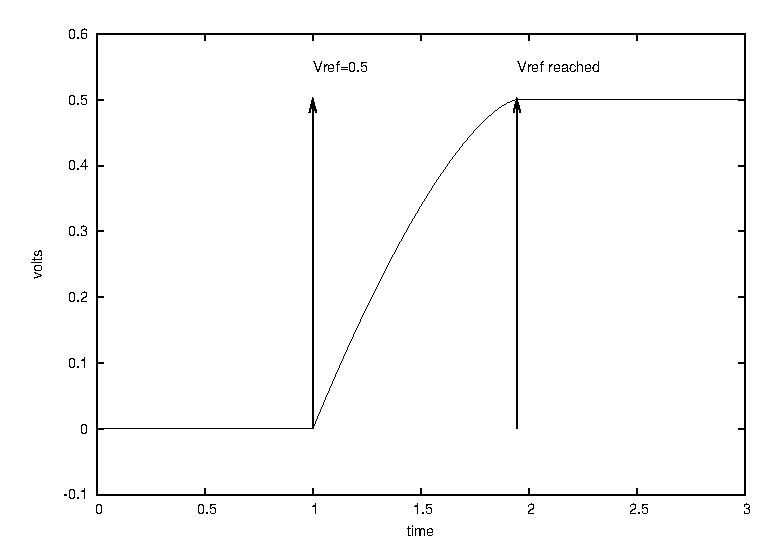
\epsfig{file=cont_models_figs/circuit.eps}
\caption{A simulation of the circuit model.}
\label{fig:circuit}
\end{figure}
